\documentclass[
	11pt, 
	DIV10,
	ngerman,
	a4paper, 
	oneside, 
	headings=normal, 
	captions=tableheading,
	final, 
	numbers=noenddot
]{scrartcl}

\usepackage{lipsum}
\usepackage{graphicx}
\usepackage{hyperref}


\title{Fully Asynchronous SPH Simulation}
\subtitle{\vspace{0.5cm}Seminar: Current Topics in Fluid Animation}
\author{Yinglun Liu}


\begin{document}
\maketitle


\section{Introduction}

Over the years, the adoption of smoothed particle hydrodynamics(SPH) has developed to become the common pratice when simulating fluids in various scenes. While iterative SPH solvers nowadays generally yield better performances, traditional non-iterative approaches do not seem to lessen in popularity due to the fact that they are easy to implement and suitable for less turbulent fluids. In these approaches, the physical state of a fluid particle is constantly influenced by its immediate neighborhood and is thus updated in each time step following a few governing equations that enforces the incompressibility of the fluid. In these equations, the computation of new attributes of the current particle requires several times the access to information from its surrounding neighbors. Intuitively, a natural practice would be to perform global updates to all particles using a single common time step.
\par
Be that as it may, a core defect of non-iterative SPH solvers lies in the lack of efficiency. To enforce a constantly negligible density deviation within the fluid, large stiffness parameters are adopted to generate high pressures. Such selection of parameters demands smaller time steps and, in turn, greater number of iterations for the sake of stable and correct particle interations. This can lead to tremendously higher overhead for the generation of visually realistic fluid animation, where tens of millions of particles are included to allow for as fine-grained details as possible.
\par
To cope with this, the author proposes a novel method for time integration of particles, in which each particle is assigned a unique time step and the whole simulation is carried out fully asynchronous. The author made the observation that, while smaller time steps are necessary in heavily populated regions to gaurantee stable simulation, in most parts of the fluid larger time steps
suffices. That is, a global time step for all particles
\section{Related Work}

This is a reference~\cite{Foley:1990}.

\section{Images and Tables}

\begin{figure}[tb]
	\centering
	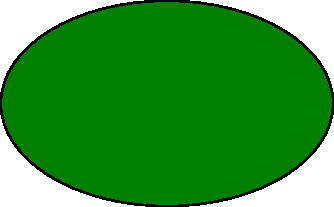
\includegraphics[width=0.5\linewidth]{images/image} 
	\caption{\label{fig:image} This is an image.
	}
\end{figure}

\begin{table}[tb]
	{
		\centering
		\begin{tabular}{|c|c|c|c|}
			\hline
			& col 1 & col 2 & col 3   \\
			\hline	
			row 1  & 1 & 2 & 3 \\
			row 2  & 4 & 5 & 6 \\
			row 3  & 7 & 8 & 9 \\
			\hline
		\end{tabular}
		\caption{\label{tab:example} This is a table.}
	}
\end{table}


Figure~\ref{fig:image} shows an example of an image.
Table~\ref{tab:example} shows an example of a table.


\bibliographystyle{alpha}
\bibliography{references}

\end{document}          
